\chapter{Développement et Conception}
\label{chapter:dev}

\label{chapitre4}
		
		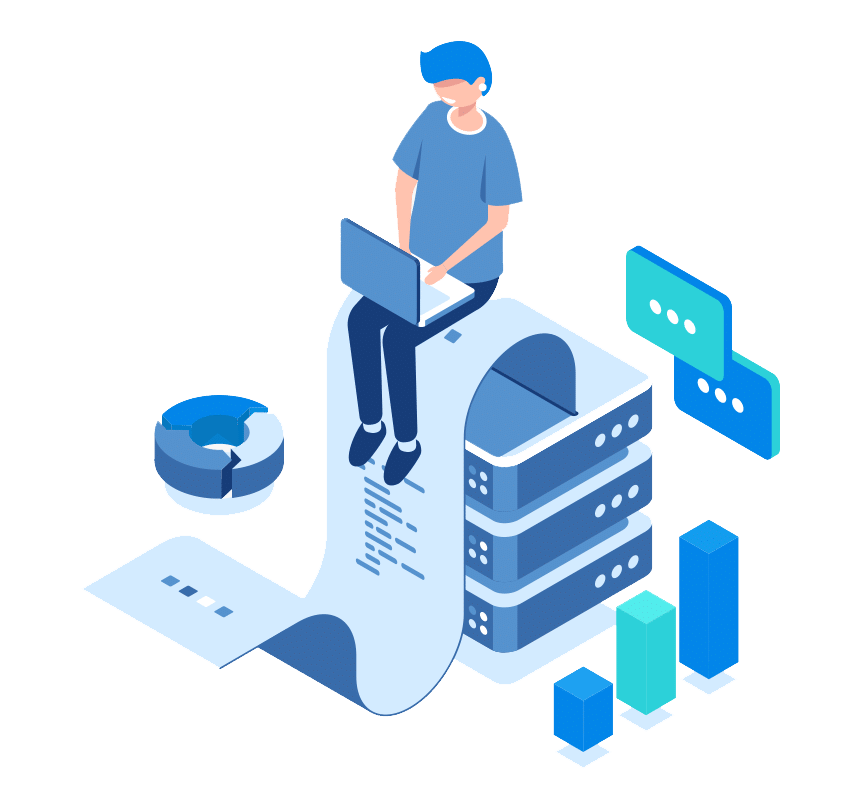
\includegraphics [width=1 \linewidth, height=0.8\textheight, keepaspectratio] {Images/chapterFigures/chFour.png}
		
	
		
		\newpage

Après avoir expliqué notre approche dans le chapitre précédent, dans ce chapitre nous expliquerons en détail comment le système proposé met en œuvre l'approche et comment elle fonctionne.

\section{Architecture du système}

Notre système se compose de plusieurs parties; une application mobile qui recueille des données, un serveur où les données en cours de traitement et stocke le résultat du traitement dans une base de données, une copie des données vers le DTP et enfin une carte interactive avec l'état de la route en temps réel pour les conducteurs (Figure \ref{fig:System}).

\subsection{Aperçu de système}
\begin{figure}[h!]
    \center
    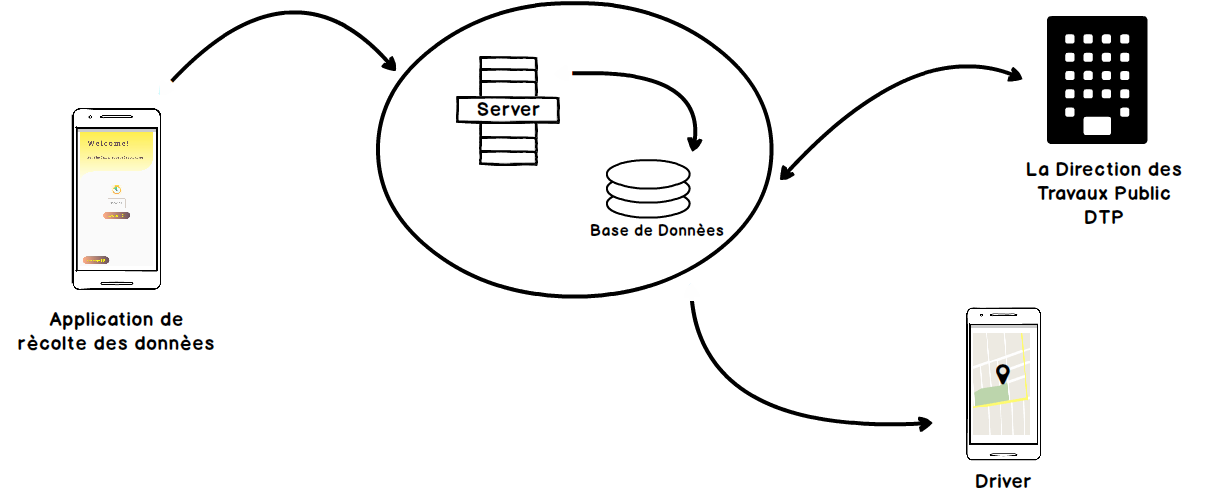
\includegraphics[width=0.75\textwidth]{Images/chapter3/systemOverview.png}
    \caption{Un aperçu du système proposé.}
    \label{fig:System}
\end{figure}

\begin{itemize}
    \item \textbf{Application de rècolte des donnèes:} Une application mobile où les capteurs du smartphone sont utilisés pour collecter les données du journal de conduite et envoyer les données au serveur.
    \item  \textbf{Server:} Après avoir reçu les données, le serveur estime l'état de la route et enregistre les résultats dans une base de données.
    \item \textbf{Base de donnèes:} Elle contient les résultats estimés de l'état de la route et l'enregistre pour être desservi par d'autres parties.
    \item  \textbf{DTP:} La Direction des Travaux Publics; la partie principale qui utilise les résultats de la base de données. Nous pouvons étendre ce système avec une application de tableau de bord pour eux, qui: \begin{itemize}
              \item Leur permettnet de surveiller régulièrement l'état de la route pour prendre plus rapidement des décisions d'entretien et de réparation.
              \item Envoyez les données fixes sur l'état de la route à la base de données après la réparation.
          \end{itemize}
    \item \textbf{Driver:} Nous pouvons également étendre ce système avec une application mobile, qui fournit au conducteur moyen une carte interactive montrant les conditions routières actuelles pour une meilleure expérience de conduite.
\end{itemize}

\subsection{Fonctionnement de système}
\begin{figure}[ht]
    \center
    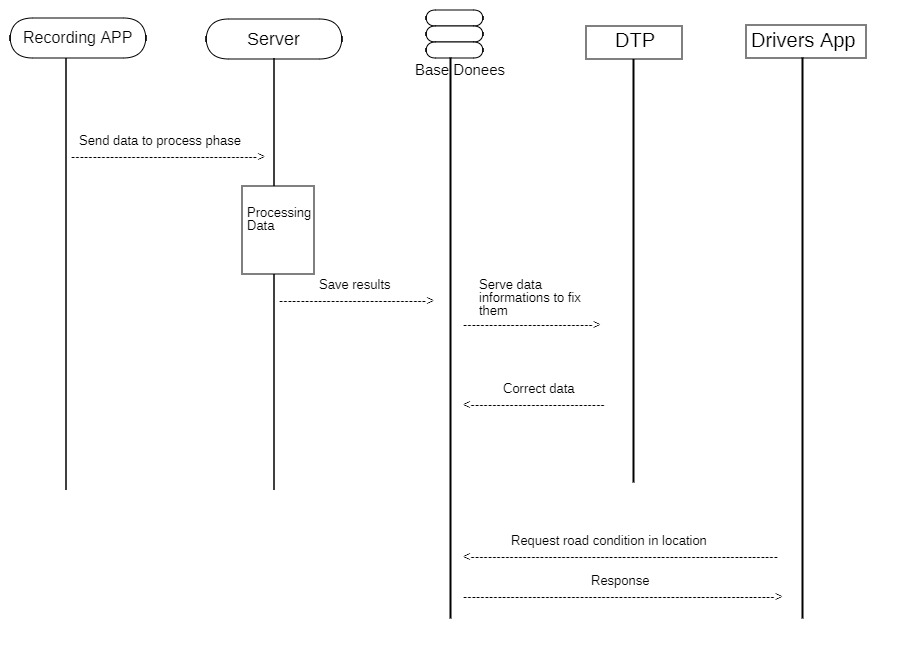
\includegraphics[width=1.2\textwidth]{Images/chapter3/diagrameSequence.jpg}
    \caption{Diagramme de séquence.}
    \label{fig:System}
\end{figure}

Notre système sous forme de diagramme montre l'envoi des données du journal de collecte de l'application d'enregistrement au serveur sous forme de fichier CSV, dès qu'il existe; Le serveur facture l'étape du processus d'enregistrement des résultats dans la base de données.

L'application de tableau de bord DTP mets à jours la base de données une fois l'anomalie corrigée, tandis que l'application Driver l'utilise pour une meilleure expérience du conducteur.



\section{Technologies utilisées}
\subsection{Python}
Python \cite{WelcomePythonOrg} est un langage de programmation qui peut être utilisé dans de nombreux contextes et est adapté à tout type d'utilisation grâce à des bibliothèques spécialisées. Il est cependant particulièrement utilisé comme langage de script pour automatiser des tâches simples mais fastidieuses. On l'utilise également comme langage de développement de prototype lorsqu'on a besoin d'une application fonctionnelle avant de l'optimiser avec un langage de plus bas niveau.

Il est particulièrement répandu dans le monde scientifique, et possède de nombreuses bibliothèques optimisées destinées aux calculs numériques \cite{PythonLangageWikipedia}.
\renewcommand{\labelitemi}{$\bullet$}

\paragraph{Pandas:}
Pandas \cite{PandasPythonData} est une bibliothèque écrite pour le langage de programmation Python permettant la manipulation et l'analyse des données. Elle propose en particulier des structures de données et des opérations de manipulation de tableaux numériques et de séries temporelles. Pandas est un logiciel libre sous licence BSD.

Les principales structures de données que propose Pandas sont les séries (pour stocker des données selon une dimension - grandeur en fonction d'un index), les DataFrames (pour stocker des données selon 2 dimensions - lignes et colonnes), les Panels (pour représenter des données selon 3 dimensions, les Panels 4D ou les Data Frames avec des index hiérarchiques aussi nommés Multi Index (pour représenter des données selon plus de 3 dimensions - hypercube) \cite{Pandas2020}.


\begin{figure}[h!]
    \center
    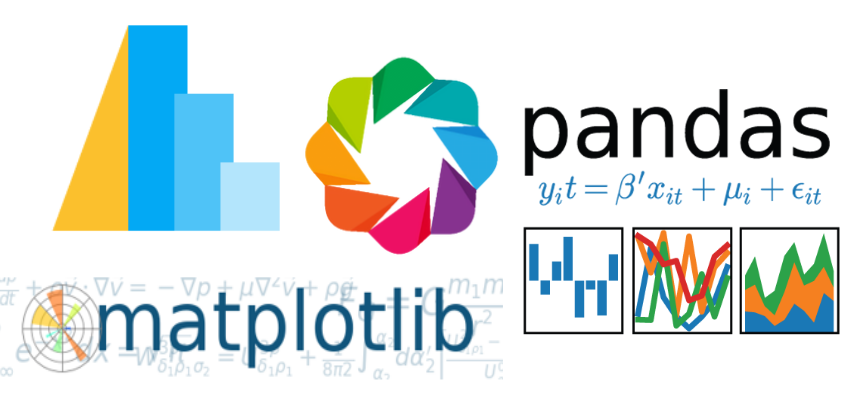
\includegraphics[width=0.50\textwidth]{Images/chapter3/python_pandas.png}
    \caption{Python et Pandas Logo.}
    \label{fig:Technologies}
\end{figure}

\subsection{REST API}
API est une abréviation de:  Application Programming Interface (ou interface de programmation d’application, en français). Pour faire simple : c’est un moyen de communication entre deux logiciels, que ce soit entre différents composants d’une application ou entre deux applications différentes.

REST ou Representational State Transfer, et constitue un ensemble de normes, ou de lignes directrices architecturales qui structurent la façon de communiquer les données entre une application et le reste du monde, ou entre différents composants de la même application.

Nous utilisons l’adjectif RESTful pour décrire les API REST. Toutes les API REST sont un type d’API – mais toutes les API ne sont pas RESTful. Les API RESTful se basent sur le protocole HTTP pour transférer les informations – le même protocole sur lequel la communication web est fondée \cite{IdentifiezAvantagesAPI}.


\subsection{Flask}
Flask \cite{WelcomeFlaskFlask} est un framework open-source de développement web en Python. Son but principal est d'être léger, afin de garder la souplesse de la programmation Python.

Flask a été créé initialement par Armin Ronacher. Le souhait de Ronacher était de réaliser un framework web contenu dans un seul fichier Python mais pouvant maintenir des applications très demandées.
En 2018, Flask était élu "Framework web le plus populaire" par le Python Developers Survey. En janvier 2020, il cumulait plus de 49000 étoiles sur Github, plus que n'importe quel autre framework de développement web Python\cite{FlaskFramework2020}.
\begin{figure}[h!]
    \center
    
\includegraphics[width=0.50\textwidth]{Images/chapter3/flask.png}
    \caption{Logo Flask.}
    \label{fig:Technologies}
\end{figure}

\subsection{Flutter}
Flutter \cite{FlutterBeautifulNative} est un SDK pour applications mobiles permettant de créer des applications hautes performances et haute fidélité pour iOS et Android à partir d’une seule base de code.
L’objectif est de permettre aux développeurs de proposer des applications hautes performances qui se sentent naturelles sur différentes plates-formes.

Comme React Native\cite{ReactNativeFramework}, Flutter fournit également des vues de style réactif( se mettent à jour automatiquement lorsque les données changent ). Flutter adopte une approche différente pour éviter les problèmes de performances causé par les autres technologies hybrides, en utilisant un langage de programmation compilé "Dart" \cite{rahmouniBindex}.
\renewcommand{\labelitemi}{$\bullet$}
\begin{itemize}
    \item \textbf{\textit{Dart:}}

          Dart est un langage de programmation polyvalent développé à l’origine par Google et ensuite approuvé en tant que norme par Ecma (ECMA-408). Il est utilisé pour créer des applications Web, serveur, bureau et mobiles.
          Dart est un langage basé sur les objets (orienté objet) qui utilise une syntaxe de style C qui transcompile éventuellement en JavaScript. \cite{WhatRevolutionaryFlutter}.
\end{itemize}
\begin{figure}[h!]
    \center
    
\includegraphics[width=0.50\textwidth]{Images/chapter3/flutter.png}
    \caption{Flutter Logo.}
    \label{fig:Technologies}
\end{figure}





\section{Application de collecte}
\label{sec:app_record}
Nous avons développé une application mobile utilisant Flutter pour la collecte de données à l'aide des capteurs de téléphone. Elle peut être utilisées comme suit :

\begin{figure}[h!]
    \begin{subfigure}{.50\textwidth}
        \center
        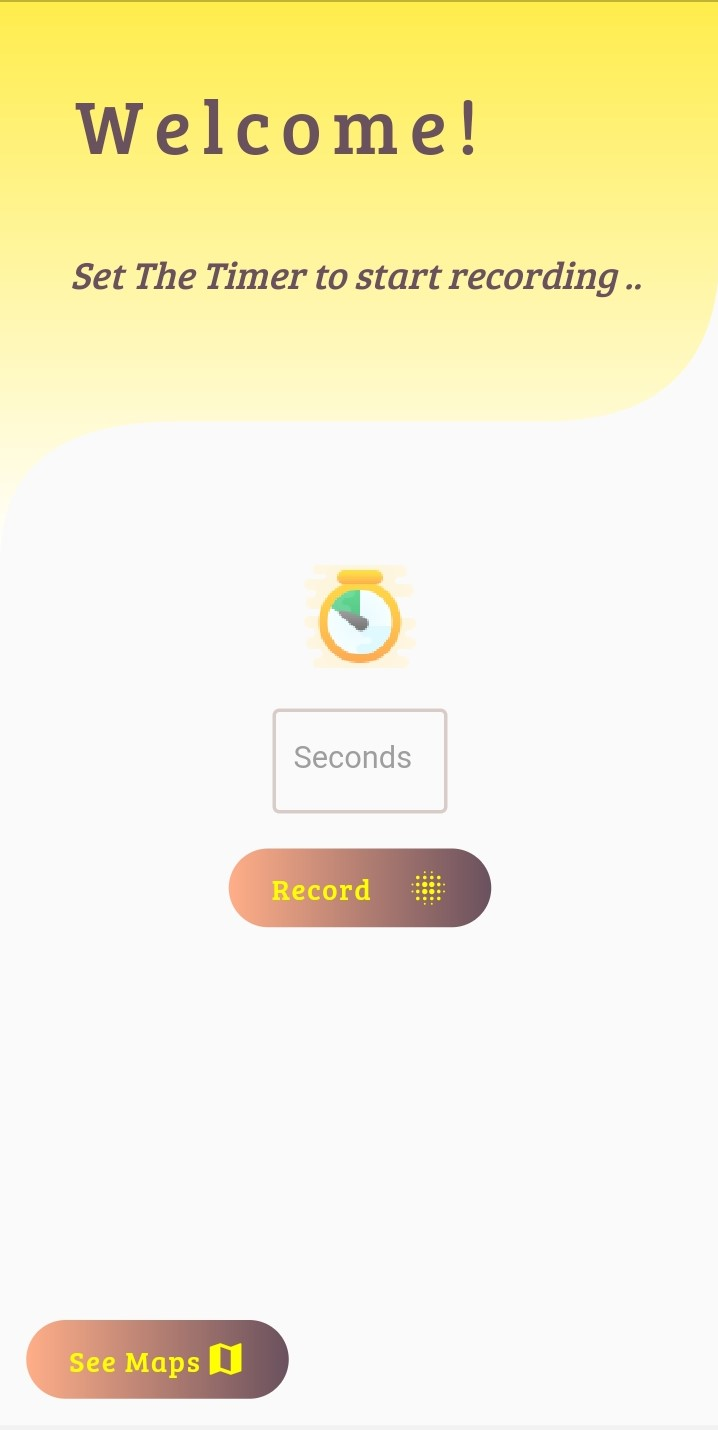
\includegraphics[width=0.50\textwidth]{Images/recordingApp/firstScreen.jpg}
        \caption{Ecran d'accueil.}
        \label{fig:Welcome Screen}
    \end{subfigure}
    \begin{subfigure}{.50\textwidth}
        \center
        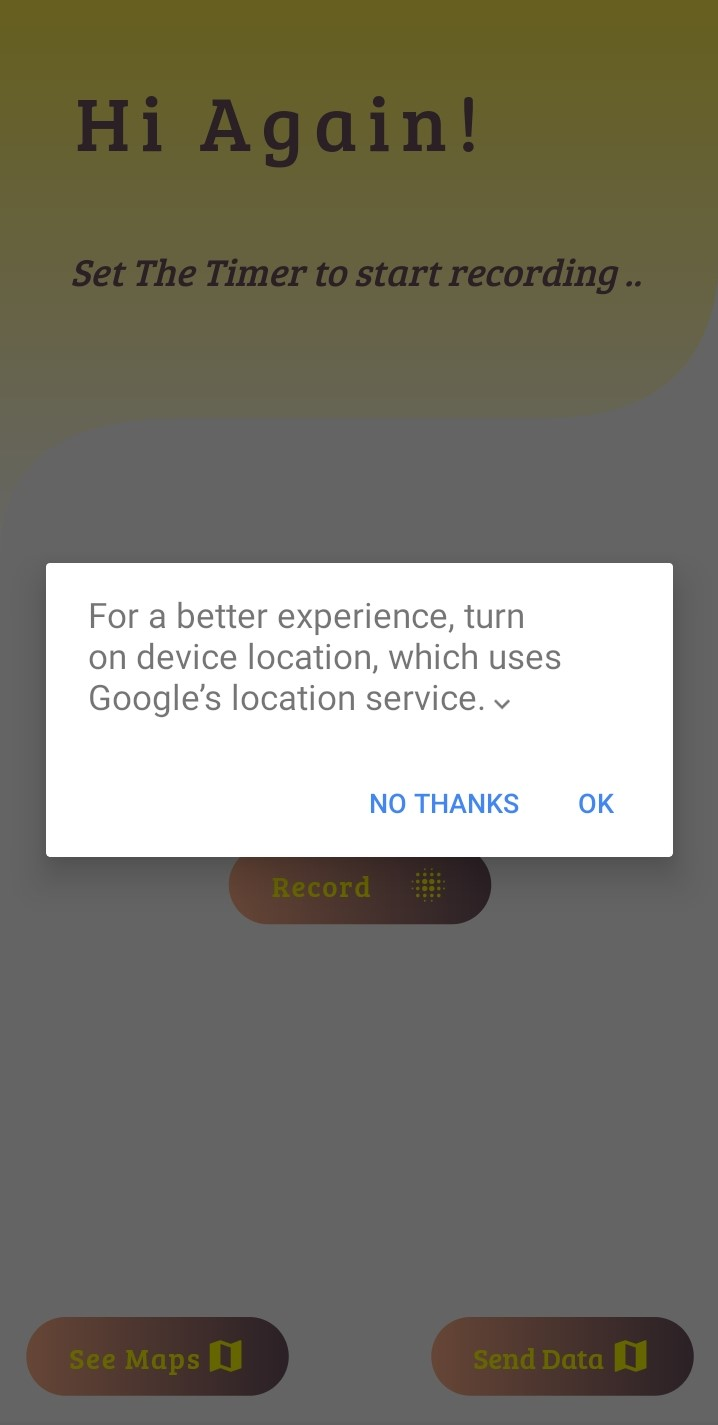
\includegraphics[width=0.50\textwidth]{Images/recordingApp/askingGps.jpg}
        \caption{Alerte d'activation GPS.}
        \label{fig:GpsAcivate}
    \end{subfigure}
    \begin{subfigure}{.50\textwidth}
        \center
        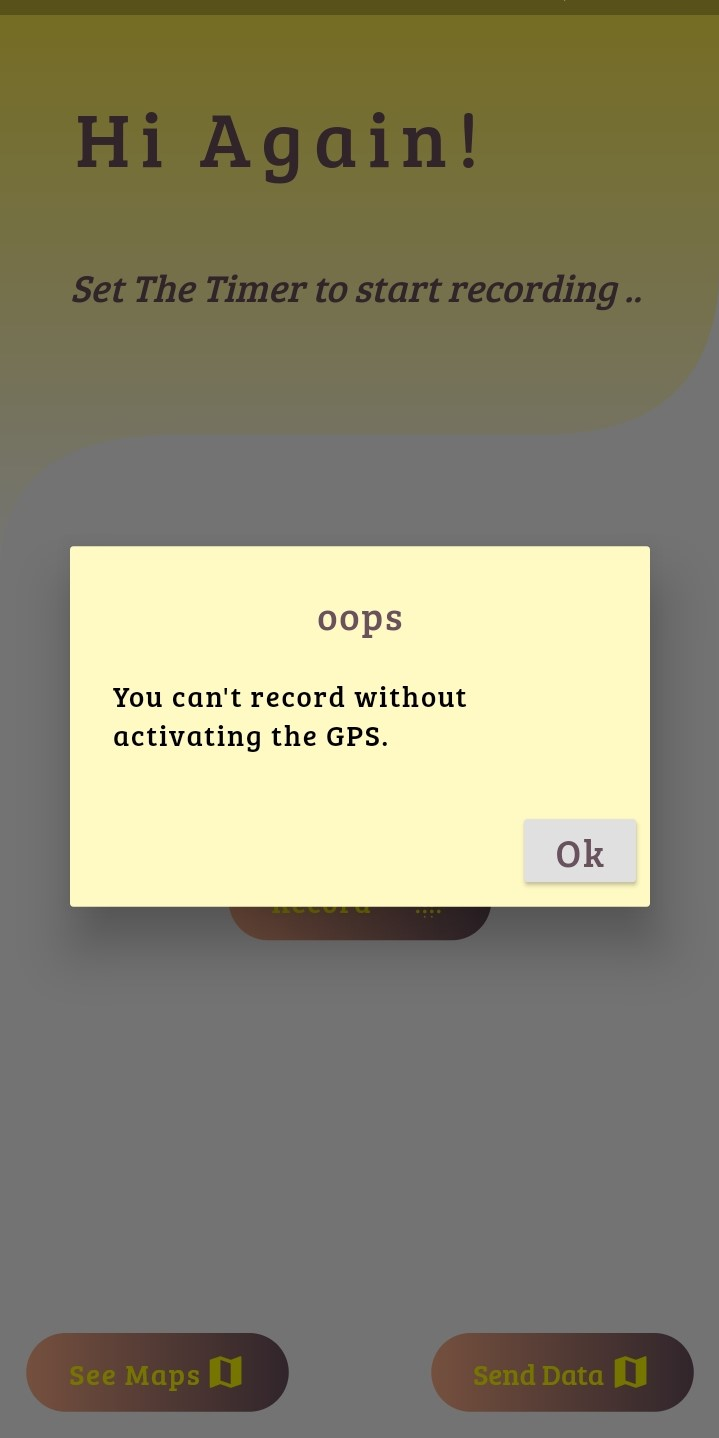
\includegraphics[width=0.50\textwidth]{Images/recordingApp/noGpsAlert.jpg}
        \caption{Notification pour activer le GPS.}
        \label{fig:gpsNotif}
    \end{subfigure}
    \begin{subfigure}{.50\textwidth}
        \center
        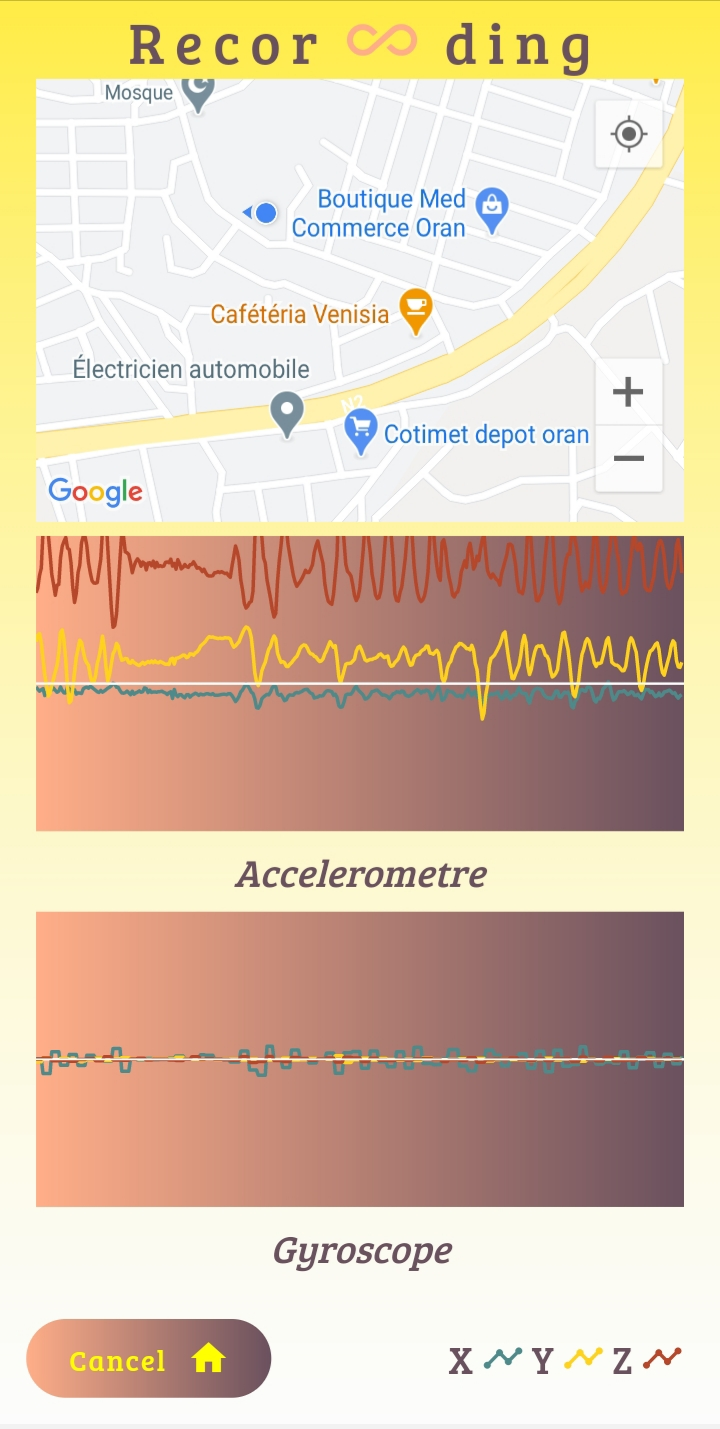
\includegraphics[width=0.50\textwidth]{Images/recordingApp/recordingScreen.jpg}
        \caption{Écran d'enregistrement.}
        \label{fig:Recording}
    \end{subfigure}
    \caption{Application de récolte.}
    \label{fig:app_recolte}
\end{figure}

\begin{itemize}
    \item D'abord, l'application demande à l'utilisateur d'entrer la durée d'enregistrement en minutes (Figure \ref{fig:Welcome Screen}).
          
    \item Deuxièmement, il lui demande d'activer le GPS (Figure \ref{fig:GpsAcivate}). Sinon, il ne démarrera pas l'enregistrement (Figure \ref{fig:gpsNotif}).
     



    \item Une fois le GPS activé et l'heure d'enregistrement entrée, l'application amène l'utilisateur à l'écran d'enregistrement, lui montrant une carte en temps réel et un graphique accéléromètre / gyroscope. Il peut annuler l'enregistrement quand il le souhaite (Figure \ref{fig:Recording}).
    
 

   

    \item Lorsque le temps est écoulé, l’utilisateur clique sur «Envoyer les données» pour que l’application envoie des données au serveur( elles seront envoyées automatiquement dans les futures versions) (Figure \ref{fig:Done}).
          \begin{figure}[h!]
              \center
              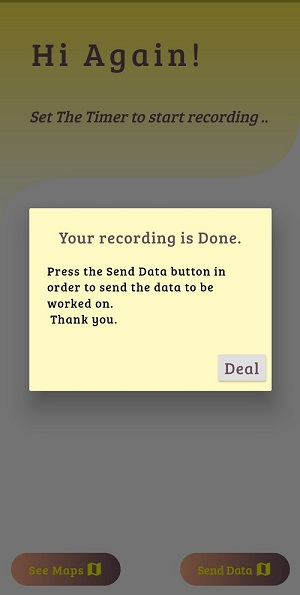
\includegraphics[width=0.50\textwidth]{Images/recordingApp/doneRecording.jpg}
              \caption{Enregistrement terminé.}
              \label{fig:Done}
          \end{figure}

          

          L'application les enregistre également sous forme de fichier CSV contenant  (Figure \ref{fig:csv}):
          \begin{itemize}
              \item La durée d'enregistrement (Time).
              \item Données de l'accéléromètre (Accel X, Accel Y, Accel Z).
              \item Données du gyroscope (Gyro X, Gyro Y, Gyro Z).
              \item Données GPS (Lat, Long).
              \item Données de la vitesse du véhicule (Speed).
          \end{itemize}
          
\begin{figure}[h!]
        \center
        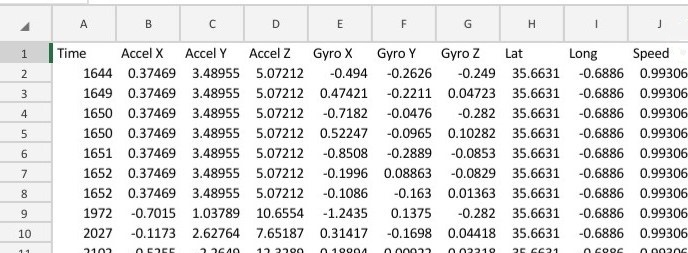
\includegraphics[width=0.95\textwidth]{Images/recordingApp/csv.jpg}
        \caption{Fichier CSV.}
        \label{fig:csv}
    \end{figure}


\end{itemize}

\newpage

\section{Serveur de traitement}
Un serveur informatique est un dispositif informatique (matériel et logiciel) qui offre des services à un ou plusieurs clients (parfois des milliers).


En fonctionnement, un serveur répond automatiquement à des requêtes provenant d'autres applications (les clients), selon le principe dit client-serveur. Le format des requêtes et des résultats est normalisé, se conforme à des protocoles réseaux et chaque service peut être exploité par tout client qui met en œuvre le protocole propre à ce service.

Dans notre implémentation, le serveur de traitement prend en charge:
\renewcommand{\labelitemi}{$\bullet$}
\begin{itemize}
    \item Le traitement des données avec l'algorithme comme indiqué dans \ref{sec:approache}, qui renvoie le Z score. 
    \item Utilise flask pour la partie de l'API, afin que toutes les autres applications concernées puissent communiquer avec le serveur, notre application principale ici est l'application Flutter \ref{sec:app_record}.
\end{itemize}
\subsection{Avantages de l'API (Application Programming Interface)}
Le server de traitement présente une API pour permettre la communication avec les autres applications. voici quelques avantages non négligeables des intégrations d'API \cite{BenefitsAPIDevelopers2019}:

\begin{figure}[h!]
    \center
    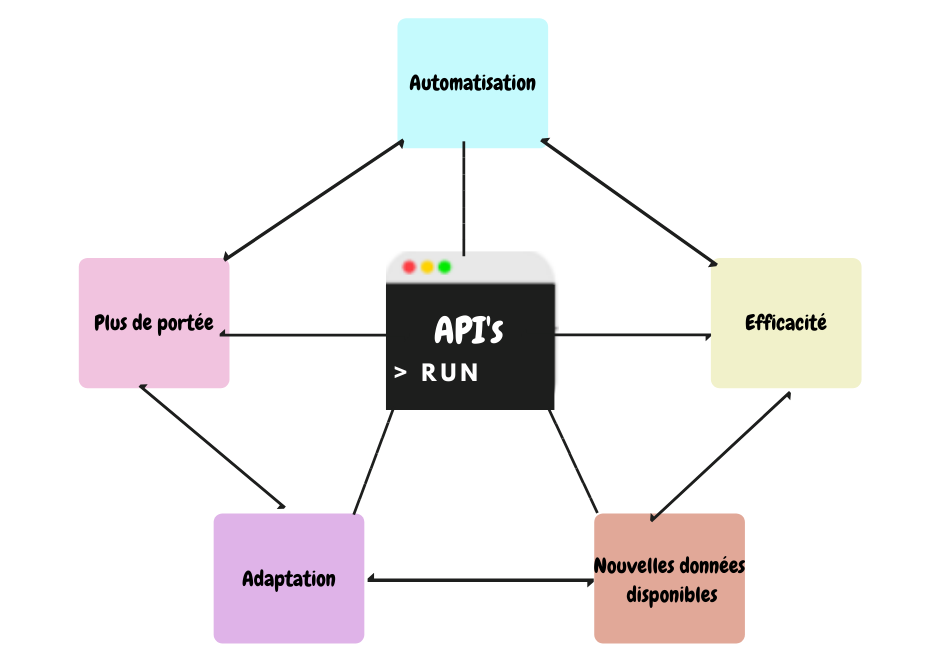
\includegraphics[width=0.75\textwidth]{Images/chapter3/apiAvantages.png}
    \caption{Avantages de l'API.}
  \end{figure}


\begin{description}
    
    \item [Plus de portée]:  En incorporant l’API dans le système, l’application peut distribuer des informations facilement à
    d’autres systèmes et peur offrir des services à de nouveaux clients (applications). La partie intéressante dans notre cas est la possibilité d'ajouter plus de fonctionnalités futures en plus du traitement de données.
     \item[Efficacité] : Une fois que vous avez accès à l'API, il est facile pour le nouveau contenu d'être publié rapidement.
     \item[Adaptation] : Chaque système doit être modifié au fil du temps, et l'API personnalisée aide à changer le système rapidement. Dans notre cas, le système (algorithme) peut être mis à jour ou complètement remplacé sans affecter les applications des clients.
     
\end{description} 

\begin{figure}[h!]
    \center
    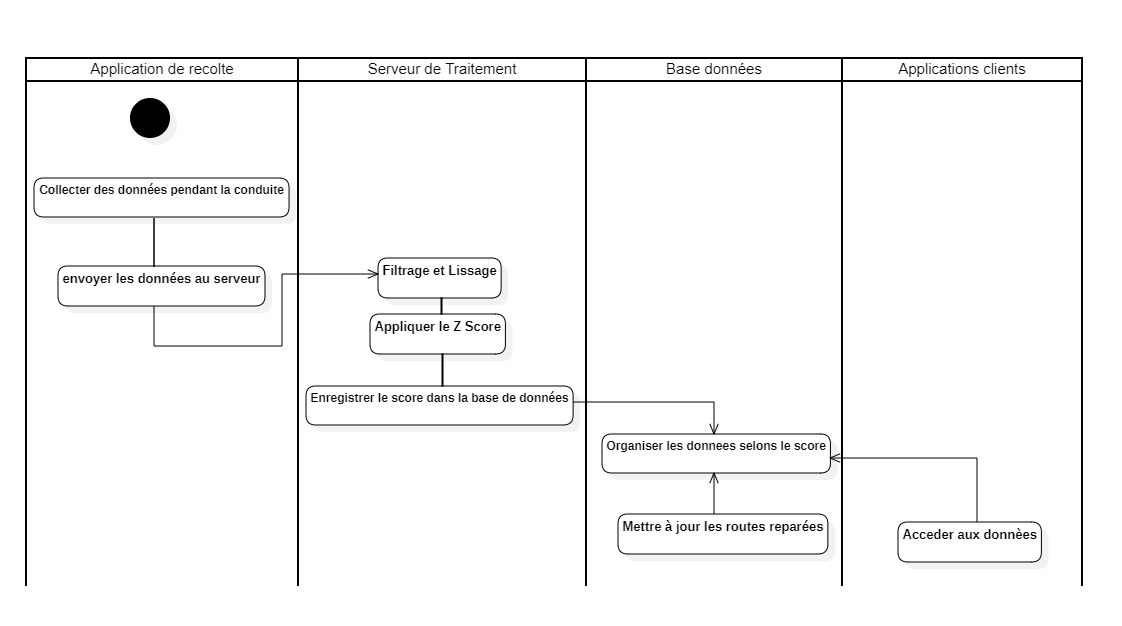
\includegraphics[width=\textwidth]{Images/chapter3/activityDiagram.png}
    \caption{Diagrame d'activités.}
    \label{activityDiagram}
  \end{figure}

  \subsection{Implémentation de l’API}
  En général, notre système suit les activités présentées dans le diagramme (\ref{activityDiagram}).
  
  
  
  Notre API travaille principalement avec deux routes:
  \begin{description}
    \item[POST /api/process\_data] : Une route qui reçoit et traite les données, puis les enregistre dans la base de données.
    \item[GET /api/road\_data] : Une route qui retourne les données stockées dans la base de données (location et score) à le application client. Elle accepte comme paramètres optionnel la position actuelle (latitude,longitude) pour retourner que les points proches de 1Km.
\end{description}

La base de données stocke le score avec un point de localisation (le centre) correspondant à la fenêtre prise, et les rend disponibles pour les différentes applications clientes.

\section{Visualisation des résultats}
Pour cette version de travail, on a essayé de visualiser les résultats obtenus depuis l’application de récolte (Figure \ref{fig:Welcome Screen}) à travers un écran Road Quality Map (Figure \ref{seeMap}) qui montre la qualité de la route de chaque 100m enregistrés à travers des cercles colorés (vert, orange, rouge), et un marqueur au centre de chaque segment avec le score correspondant. Pour plus de visibilité, les cercles verts qui représentent les segments de bonne qualité sont
cachés par défaut.

\newpage
\begin{figure}[h!]
    \center
    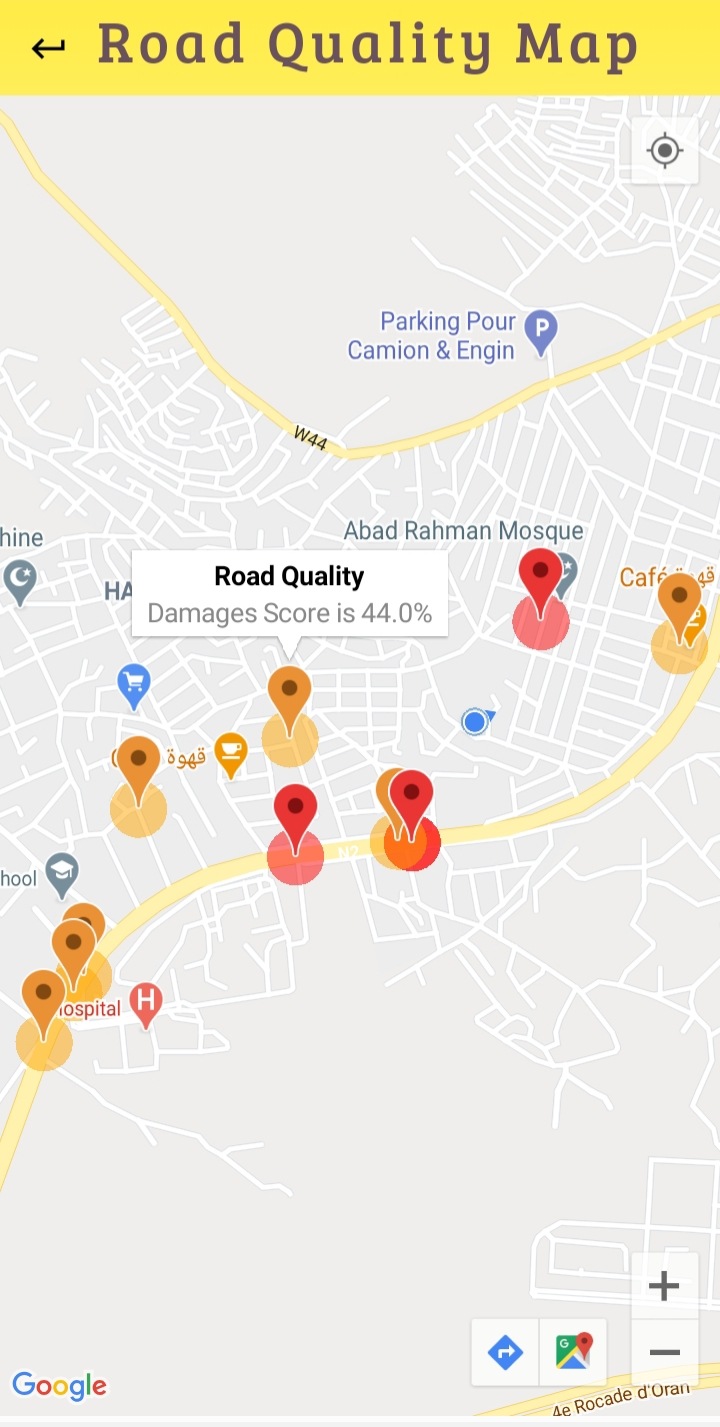
\includegraphics[width=0.50\textwidth]{Images/recordingApp/seeMap.jpg}
    \caption{Visualisation des résultats sur la carte.}
    \label{seeMap}
  \end{figure} 



\section{Conclusion}
Dans ce chapitre, nous avons décrit l'architecture de notre système, et les différentes technologies utilisées pour ce travail, nous avons également présenté comment l'application de collecte est construite et comment le serveur communique avec les différents parties. Concernant la partie base de données, elle est prévue dans les travaux futurs. Malgré les différentes contraintes (complexité du problème, manque de données claires, Pandémie actuelle), la représentation choisie pour cette première version reste suffisante et facilement extensible pour de futures améliorations.



